\documentclass[a4paper,10pt,twocolumn,oneside]{article}
\setlength{\columnsep}{10pt}                                                              %兩欄模式的間距
\setlength{\columnseprule}{0pt}                                                                %兩欄模式間格線粗細

\usepackage{amsthm}								%定義,例題
\usepackage{amssymb}
%\usepackage[margin=2cm]{geometry}
\usepackage{fontspec}								%設定字體
\usepackage{color}
\usepackage[x11names]{xcolor}
\usepackage{listings}								%顯示code用的
%\usepackage[Glenn]{fncychap}						%排版,頁面模板
\usepackage{fancyhdr}								%設定頁首頁尾
\usepackage{graphicx}								%Graphic
\usepackage{enumerate}
\usepackage{titlesec}
\usepackage{amsmath}
\usepackage{tikz}
\usepackage{xpatch}
\usepackage[CheckSingle, CJKmath]{xeCJK}
\usepackage{CJKulem}
\usepackage[T1]{fontenc}
%\titlespacing{\section}{0cm}{0cm}{0cm}
%\titlespacing{\subsection}{0cm}{0cm}{0cm}
\usepackage{amsmath, courier, listings, fancyhdr, graphicx}
\topmargin=0pt
\headsep=5pt
\textheight=780pt
%\footskip=0pt
\voffset=-40pt
\textwidth=545pt
\marginparsep=0pt
\marginparwidth=0pt
\marginparpush=0pt
\oddsidemargin=0pt
\evensidemargin=0pt
\hoffset=-42pt

%\renewcommand\listfigurename{圖目錄}
%\renewcommand\listtablename{表目錄} 

%%%%%%%%%%%%%%%%%%%%%%%%%%%%%

%\setmainfont {Consolas}			%主要字型
  

%\setmonofont{Monaco} 

% \setmainfont{TeX Gyre Termes}
\setmainfont{Consolas}				%主要字型
\setmonofont{Monaco}				%主要字型
%\setCJKmainfont{Noto Sans CJK TC}

\setCJKmainfont{微軟正黑體}			%中文字型
%\setmainfont{sourcecodepro}
%\XeTeXlinebreaklocale "zh"						%中文自動換行
%\XeTeXlinebreakskip = 0pt plus 1pt				%設定段落之間的距離
\setcounter{secnumdepth}{3}						%目錄顯示第三層

%%%%%%%%%%%%%%%%%%%%%%%%%%%%%
\makeatletter
\lst@CCPutMacro\lst@ProcessOther {"2D}{\lst@ttfamily{-{}}{-{}}}
\@empty\z@\@empty
\makeatother
\lstset{											% Code顯示
language=C++,										% the language of the code
basicstyle=\footnotesize\ttfamily, 						% the size of the fonts that are used for the code
%numbers=left,										% where to put the line-numbers
numberstyle=\footnotesize,						% the size of the fonts that are used for the line-numbers
stepnumber=1,										% the step between two line-numbers. If it's 1, each line  will be numbered
numbersep=5pt,										% how far the line-numbers are from the code
backgroundcolor=\color{white},					% choose the background color. You must add \usepackage{color}
showspaces=false,									% show spaces adding particular underscores
showstringspaces=false,							% underline spaces within strings
showtabs=false,									% show tabs within strings adding particular underscores
frame=false,											% adds a frame around the code
tabsize=2,											% sets default tabsize to 2 spaces
captionpos=b,										% sets the caption-position to bottom
breaklines=true,									% sets automatic line breaking
breakatwhitespace=false,							% sets if automatic breaks should only happen at whitespace
escapeinside={\%*}{*)},							% if you want to add a comment within your code
morekeywords={*},									% if you want to add more keywords to the set
keywordstyle=\bfseries\color{Blue1},
commentstyle=\itshape\color{Red4},
stringstyle=\itshape\color{Green4},
}

%%%%%%%%%%%%%%%%%%%%%%%%%%%%%

\begin{document}
\pagestyle{fancy}
%\fancyfoot{}
%\fancyfoot[R]{\includegraphics[width=20pt]{ironwood.jpg}}
\fancyhead[L]{National Taiwan Ocean University XwX Team}
\fancyhead[R]{\thepage}
\renewcommand{\headrulewidth}{0.4pt}
\renewcommand{\contentsname}{Contents} 

\scriptsize
\tableofcontents
%%%%%%%%%%%%%%%%%%%%%%%%%%%%%

% \newpage

\section{Basic}

\subsection{default code}
\lstinputlisting{basic/default.cpp}

\subsection{.vimrc}
\lstinputlisting{basic/vimrc_warner}

\subsection{Increase Stack Size (linux)}
\lstinputlisting{basic/IncStack.cpp}

% \subsection{Increase Stack Size}
% \lstinputlisting{basic/IncStack_windows.cpp}

\subsection{Misc}
\lstinputlisting{basic/misc.cpp}

\subsection{check}
\lstinputlisting{basic/run.sh}

\subsection{python-related}
\lstinputlisting{basic/pythonBasic.py}

% \subsection{java-related}
% \lstinputlisting{basic/java-related.java}

\section{flow}

\subsection{ISAP $O(V^{3})$}
\lstinputlisting{flow/isap.cpp}

\subsection{MinCostFlow}
\lstinputlisting{flow/zkwflow.cpp}

\subsection{Dinic $O(V^{2}E)$}
\lstinputlisting{flow/dinic_BCW.cpp}

%\subsection{Hungarian}
%\lstinputlisting{flow/Hungarian.cpp}

%\subsection{Hungarian Unbalanced}
%\lstinputlisting{flow/HungarianUnbalanced.cpp}

\subsection{Kuhn Munkres 最大完美二分匹配 $O(n^{3})$}
\lstinputlisting{flow/KM2.cpp}

%\subsection{Directed MST}
%\lstinputlisting{flow/DMST.cpp}

\subsection{SW min-cut (不限S-T的min-cut) $O(V^{3})$}
\lstinputlisting{flow/SW-mincut.cpp}

% \subsection{Max Cost Circulation}
% \lstinputlisting{flow/MaxCostCirculation.cpp}

%\subsection{Gusfield}
%\lstinputlisting{flow/gusfield.cpp}

\subsection{Max flow with lower/upper bound}
\lstinputlisting{flow/BoundedMaxflow.cpp}

% \subsection{Relabel to Front}
% \lstinputlisting{flow/relabelToFront.cpp}

% \subsection{HLPPA (稠密圖flow)}
% \lstinputlisting{flow/HLPPA2.cpp}

\subsection{Flow Method}
\lstinputlisting[language={[LaTeX]TeX},mathescape]{flow/FlowMethod.tex}


% \lstinputlisting{flow/FlowMethod.tex}

\section{Math}
\subsection{FFT}
\lstinputlisting{math/FFT.cpp}

%\subsection{NTT}
%\lstinputlisting{math/ntt.cpp}

%\subsection{Fast Walsh Transform}
%\lstinputlisting{math/FWT.cpp}

%\subsection{Poly operator}
%\lstinputlisting{math/PolyOp_new.cpp}

\subsection{O(1)mul}
\lstinputlisting{math/O(1)mul.cpp}

% \subsection{BigInt}
% \lstinputlisting{math/Bigint_full.cpp}

%\subsection{Linear Recurrence}
%\lstinputlisting{math/linearRecurrence.cpp}

% \subsection{Simplex 線性規劃}
% \lstinputlisting{math/Simplex.cpp}

\subsection{Faulhaber ($\sum\limits_{i=1}^{n}i^p$)}
\lstinputlisting{math/Faulhaber.cpp}

\subsection{Chinese Remainder}
\lstinputlisting{math/chineseRemainder.cpp}

\subsection{Miller Rabin}
\lstinputlisting{math/Miller_Rabin.cpp}

\subsection{Pollard Rho}
\lstinputlisting{math/pollardRho.cpp}

\subsection{Josephus Problem}
\lstinputlisting{math/Josephus.cpp}

%\subsection{Poly Generator}
%\lstinputlisting{math/PolyGen.cpp}

%\subsection{Matrix Pseudo Inverse}
%\lstinputlisting{math/Square_Matrix_pinv.cpp}

\subsection{Matrix}
\lstinputlisting{math/matrix.cpp}

\subsection{Gaussian Elimination}
\lstinputlisting{math/gauss.cpp}

\subsection{Inverse Matrix}
\lstinputlisting{math/inverse_matrix.cpp}


\subsection{模反元素}
\lstinputlisting{math/mod_reverse.cpp}

\subsection{ax+by=gcd}
\lstinputlisting{math/ax+by=gcd.cpp}

\subsection{Discrete sqrt}
\lstinputlisting{math/DiscreteSqrt.cpp}

% \subsection{SchreierSims}
% \lstinputlisting{math/SchreierSims.cpp}

%\subsection{Romberg 定積分}
%\lstinputlisting{math/Romberg.cpp}

%\subsection{Discrete K-th sqrt}
%\lstinputlisting{math/DiscreteKthsqrt.cpp}

\subsection{Prefix Inverse}
\lstinputlisting{math/prefixInv.cpp}

\subsection{Roots of Polynomial 找多項式的根}
\lstinputlisting{math/rootsOfPolynomial.cpp}

\subsection{Combination thearom}
\lstinputlisting{math/Combination_thearom.cpp}

% \subsection{inverse}
% \lstinputlisting{math/inverse.cpp}

%\subsection{Mod}
%\lstinputlisting{math/MOD.cpp}

\subsection{Primes}
\lstinputlisting{math/primes.cpp}

\subsection{Phi}
\lstinputlisting{math/phi.cpp}

\subsection{Result}
\begin{itemize}
\item Lucas’ Theorem :\\
  For $n, m \in \mathbb{Z}^{*}$ and prime $P$,
  $C(m,n) \mod P$
  %= C(\frac{m}{M},n/M) * C(m\%M,n\%M) mod P
	$= \Pi ( C(m_i,n_i) )$
  where $m_i$ is the $i$-th digit of $m$ in base $P$.
\item Stirling approximation : \\
  $n!\approx\sqrt{ 2 \pi n}(\frac{n}{e})^{n}e^\frac{1}{12n}$
\item Stirling Numbers(permutation $|P|=n$ with $k$ cycles): \\
  $S(n,k) = \text{coefficient of }x^k \text{ in } \Pi_{i=0}^{n-1} (x+i)$
\item Stirling Numbers(Partition $n$ elements into $k$ non-empty set): \\
  $S(n,k) = \frac{1}{k!} \sum\limits_{j=0}^k (-1)^{k-j} {k \choose j} j^n$
\item Pick’s Theorem : $A = i + b/2 - 1$\\
	在二維座標平面中畫上網格,對於任何簡單多邊形\\
  $A$: 面積、 $i$: 內部的格點數、 $b$: 邊上的格點數
\item Catalan number : $C_n = {2n \choose n}/(n+1)$\\
  $C^{n+m}_{n}-C^{n+m}_{n+1} = (m+n)! \frac{n-m+1}{n+1}\quad for \quad  n \ge m$\\
  $C_n = \frac{1}{n+1}{2n \choose n} = \frac{(2n)!}{(n+1)!n!}$\\
  $C_0 = 1 \quad  and \quad C_{n+1}= 2(\frac{2n+1}{n+2})C_n$\\
  $C_0 = 1 \quad  and \quad C_{n+1} = \sum_{i=0}^{n} C_iC_{n-i} \quad for \quad  n \ge 0$
\item Euler Characteristic: \\
  planar graph: $V-E+F-C=1$ \\
  convex polyhedron: $V-E+F=2$ \\
  $V,E,F,C$: number of vertices, edges, faces(regions), and components
\item Kirchhoff's theorem : \\
  $A_{ii} = deg(i), A_{ij} = (i,j) \in E\ ? -1 : 0$,
  Deleting any one row, one column, and cal the det(A)
\item Polya' theorem ($c$ is number of color,$m$ is the number of cycle size): \\
  $(\sum_{i=1}^{m}{c^{gcd(i,m)}})/m$
\item Burnside lemma: \\
  $|X/G| = \frac{1}{|G|}\sum\limits_{g\in G} |X^g|$
\item 錯排公式 :  ($n$個人中,每個人皆不再原來位置的組合數): \\
  $dp[0]=1;dp[1]=0;$\\
  $dp[i]=(i-1)*(dp[i-1]+dp[i-2])$;
\item Bell數 (有$n$個人,把他們拆組的方法總數) : \\
  $B_0= 1$\\
  $B_n= \sum_{k=0}^{n} s(n,k)\quad (second-stirling)\\
  B_{n+1}= \sum_{k=0}^{n}{n \choose k} B_k$
\item Wilson's theorem :\\
  $(p-1)! \equiv -1 (mod \ p)$
\item Fermat's little theorem :\\
  $a^p \equiv a (mod \ p)$
\item Euler's totient function:\\
  $ A ^ {B ^ C} mod \ p = pow(A,pow(B,C,p-1)) mod \ p$
\item 歐拉函數降冪公式:\\
  $A^B \mod C=A^{B \mod \phi(c) + \phi(c)}\mod C$
\item 用歐拉函數求模反元素:\\
  如果$a$和$n$互質,則$a$對$n$的模反元素\\
  $a^{-1 }\equiv a^{\phi(n)-1 }(mod \ n)$
\item 6的倍數: \\
 $(a-1)^3 + (a+1)^3 + (-a)^3 + (-a)^3 = 6a$
\item 上高斯(向上取整):\\
  $\lceil \frac{a}{b} \rceil = \frac{a+b-1}{b}$\\
\item 卡塔蘭數:\\
  $C_n = \frac{1}{n+1} {2n \choose n} = \frac{(2n)!}{(n+1)!n!}$
\end{itemize}



\section{Geometry}

% \subsection{Points class}
% \lstinputlisting{geometry/Points.cpp}

\subsection{definition}
\lstinputlisting{geometry/definition.cpp}

\subsection{Intersection of 2 lines}
\lstinputlisting{geometry/Intersection_of_two_lines.cpp}

% \lstinputlisting{geometry/halfPlaneIntersection.cpp}
\subsection{halfPlaneIntersection}
\lstinputlisting{geometry/Half_plane_intersection.cpp}

\subsection{Convex Hull}
\lstinputlisting{geometry/convex_hull.cpp}

\subsection{Convex Hull trick}
\lstinputlisting{geometry/ConvexHulltrick.cpp}

%\subsection{Convex Hull 3D}
%\lstinputlisting{geometry/Convexhull3D.cpp}

\subsection{Intersection of 2 segments}
\lstinputlisting{geometry/Intersection_of_two_segments.cpp}

%\subsection{Intersection of circle and segment}
%\lstinputlisting{geometry/Intersection_of_circle_and_segment.cpp}

%\subsection{Intersection of polygon and circle}
%\lstinputlisting{geometry/Intersection_of_polygon_and_circle2.cpp}

\subsection{Point In Polygon}
\lstinputlisting{geometry/pointInPolygon.cpp}

%\subsection{Intersection of 2 circles}
%\subsection{Circle cover}
%\lstinputlisting{geometry/CircleCover.cpp}

%\subsection{Li Chao Segment Tree}
%\lstinputlisting{dataStructure/LiChaoST.cpp}

\subsection{Tangent line of two circles}
\lstinputlisting{geometry/Tangent_line_of_two_circles.cpp}


\subsection{Minimum distance of two convex}
\lstinputlisting{geometry/minDistOfTwoConvex.cpp}

%\subsection{KD Tree}
%\lstinputlisting{geometry/KD_Tree.cpp}
%\lstinputlisting{geometry/KD_Tree1.cpp}

%\subsection{Poly Union}
%\lstinputlisting{geometry/polyUnion.cpp}

%\subsection{Lower Concave Hull}
%\lstinputlisting{geometry/lowerConcaveHull3.cpp}

% \subsection{Delaunay Triangulation}
% \lstinputlisting{geometry/DelaunayTriangulation.cpp}

%\subsection{Min Enclosing Circle}
%\lstinputlisting{geometry/mec.cpp}

%\subsection{Min Enclosing Ball}
%\lstinputlisting{geometry/minEnclosingBall.cpp}

%\subsection{Minkowski sum}
%\lstinputlisting{geometry/Minkowski_Sum.cpp}

%\subsection{Minkowski sum}
%\lstinputlisting{geometry/minkowski-convex-hull.cpp}

% \subsection{Min Enclosing Circle}
% \lstinputlisting{geometry/minEnclosingCircle.cpp}

%\subsection{Min/Max Enclosing Rectangle}
%\lstinputlisting{geometry/minMaxEnclosingRectangle.cpp}

%\subsection{Li Chao Segment Tree}
%\lstinputlisting{geometry/LiChaoST.cpp}

\subsection{Area of Rectangles}
\lstinputlisting{geometry/Area_of_Rectangles.cpp}

\subsection{Min dist on Cuboid}
\lstinputlisting{geometry/minDistonCuboid.cpp}

\subsection{Heart of Triangle}
\lstinputlisting{geometry/triangle.cpp}

\section{Graph}

%\subsection{DominatorTree}
%\lstinputlisting{graph/DominatorTree.cpp}

\subsection{DSU 並查集 \& MST}
\lstinputlisting{graph/DSU.cpp}

\subsection{Lowest Common Ancestor $O(lgn)$}
\lstinputlisting{graph/LCA.cpp}

\subsection{Hamiltonian path $O(n^{2}2^{n})$}
\lstinputlisting{graph/Hamiltonian_path.cpp}

\subsection{MaximumClique 最大團}
% \lstinputlisting{graph/MaxClique.cpp}
\lstinputlisting{graph/MaximumClique.cpp}

\subsection{MaximalClique 極大團}
% \lstinputlisting{graph/MaxClique.cpp}
\lstinputlisting{graph/MaximalClique.cpp}

%\subsection{Number of Maximal Clique}
%\lstinputlisting{graph/NumberofMaximalClique.cpp}

%\subsection{Centroid Decomposition}
%\lstinputlisting{graph/CentroidDecomposition2.cpp}

\subsection{BCC based on vertex 點雙聯通分量}
\lstinputlisting{graph/bcc_vertex.cpp}

\subsection{Strongly Connected Component 強連通分量}
\lstinputlisting{graph/kosaraju.cpp}

%\subsection{Dynamic MST}
%\lstinputlisting{graph/DynamicMST.cpp}

\subsection{Maximum General graph Matching}
\lstinputlisting{graph/generalMatching.cpp}

%\subsection{Minimum General Weighted Matching}
%\lstinputlisting{graph/Minimum_General_Weighted_Matching.cpp}

%\subsection{Maximum General Weighted Matching}
%\lstinputlisting{graph/BorrowedGeneralWeightedMatching.cpp}

%\subsection{Minimum Steiner Tree}
%\lstinputlisting{graph/MinimumSteinerTree.cpp}

%\newpage
\subsection{Min Mean Cycle}
\lstinputlisting{graph/MinMeanCycle.cpp}

\subsection{Directed Graph Min Cost Cycle}
\lstinputlisting{graph/DirectedGraphMinCycle.cpp}

\subsection{K-th Shortest Path}
\lstinputlisting{graph/KSP.cpp}

\subsection{Floryd Warshall}
\lstinputlisting{graph/FlorydWarshall.cpp}

\subsection{SPFA}
\lstinputlisting{graph/spfa.cpp}

\subsection{Tree Hash}
\lstinputlisting{graph/treehash.cpp}

\subsection{HeavyLightDecomposition}
\lstinputlisting{graph/HeavyLightDecomp.cpp}

\subsection{差分約束}
約束條件 $V_j-V_i\le W$ addEdge($V_i, V_j, W $) and run bellman-ford or spfa
%\\[3cm]

%\subsection{Graph Hash}
%$$F_t(i) = 
  (F_{t-1}(i) \times A + 
  \sum_{i\rightarrow j} F_{t-1}(j) \times B + 
  \sum_{j\rightarrow i} F_{t-1}(j) \times C +
  D \times (i = a))\ mod\ P
$$
for each node i, iterate t times.
t, A, B, C, D, P are hash parameter


% \subsection{eulerPath}
% \lstinputlisting{graph/eulerPath.cpp}

\section{String}

\subsection{PalTree $O(n)$}
\lstinputlisting{string/PalTree2.cpp}

%\subsection{SuffixArray}
%\lstinputlisting{string/Suffix_Array.cpp}

\subsection{Longest Increasing Subsequence}
\lstinputlisting{string/LIS.cpp}


\subsection{Longest Common Subsequence $O(nlgn)$}
\lstinputlisting{string/LCS.cpp}

\subsection{KMP}
\lstinputlisting{string/KMP.cpp}

\subsection{SAIS $O(n)$}
\lstinputlisting{string/SAIS.cpp}

%\subsection{SuffixAutomata}
%\lstinputlisting{string/SAM.cpp}

\subsection{Z Value $O(n)$}
\lstinputlisting{string/zvalue.cpp}

%\subsection{BWT}
%\lstinputlisting{string/BWT.cpp}

\subsection{Manacher Algorithm $O(n)$}
\lstinputlisting{string/zvalue_palindrome.cpp}

\subsection{Smallest Rotation}
\lstinputlisting{string/minRotation.cpp}

%\subsection{Baker Bird}
%\lstinputlisting{string/bakerBird.cpp}

\subsection{Cyclic LCS}
\lstinputlisting{string/cyclicLCS.cpp}

\subsection{Hash}
 \lstinputlisting{string/hash.cpp}


\section{Data Structure}

\subsection{Segment tree}
\lstinputlisting{dataStructure/seg_treewithtestcase.cpp}

\subsection{持久化 SMT}
\lstinputlisting{dataStructure/SegmentTree_pointer.cpp}

\subsection{Trie}
\lstinputlisting{dataStructure/trie.cpp}

\subsection{Treap  (interval reverse)}
\lstinputlisting{dataStructure/treap_split_key&kth.cpp}

\subsection{Treap  (interval erase)}
\lstinputlisting{dataStructure/treap_erase.cpp}

\subsection{Link-Cut Tree}
\lstinputlisting{dataStructure/link_cut_tree.cpp}

\subsection{BIT}
\lstinputlisting{dataStructure/BIT.cpp}

% \subsection{Disjoint Set}
% \lstinputlisting{dataStructure/DisjointSet1.cpp}

%\subsection{Pairing Heap}
%\lstinputlisting{dataStructure/pairing_heap.cpp}

%\subsection{Leftist Heap}
%\lstinputlisting{dataStructure/Leftist_Heap.cpp}

\subsection{Black Magic}
\lstinputlisting{dataStructure/extc_bt.cpp}

%\newpage
\section{Others}

\subsection{SOS dp}
\lstinputlisting{others/SOS_dp.cpp}

%\subsection{Number of Occurrences of Digit}
%\lstinputlisting{others/numberCount.cpp}

%\subsection{Find max tangent(x,y is increasing)}
%\lstinputlisting{others/maxtan.cpp}

%\subsection{Exact Cover Set}
%\lstinputlisting{others/exactCoverSet.cpp}

%\subsection{Hibert Curve}
%\lstinputlisting{others/HibertCurve.cpp}

\subsection{De Brujin sequence}
\lstinputlisting{others/DeBrujin.cpp}

\subsection{CDQ 分治}
\lstinputlisting{others/CDQ.cpp}

\subsection{3D LIS}
\lstinputlisting{others/3D-LIS.cpp}

%\newpage
\subsection{Ternary Search}
\lstinputlisting{others/TernarySearch.cpp}

\subsection{Max Subrectangle}
\lstinputlisting{others/max_subrectangle.cpp}

\subsection{Maximal Rectangle}
\lstinputlisting{others/maximalRectangle.cpp}

\subsection{p-Median}
\lstinputlisting{others/pMedian.cpp}

\subsection{Tree Knapsack}
\lstinputlisting{others/treeKnapsack.cpp}

\subsection{AC-Automaton}
 \lstinputlisting{string/AC-Automaton.cpp}

% \subsection{Aho-Corasick}
% \lstinputlisting{string/Aho-Corasick.cpp}

%\subsection{\# of Intersection of segments}
%\lstinputlisting{others/painter.cpp}

% \lstinputlisting{others/funny.cpp}
% \centering

%\begin{figure}[htbp]%H为当前位置,!htb为忽略美学标准,htbp为浮动图形
%\includegraphics[width=0.4\textwidth]{others/AC.png} %插入图片,[]中设置图片大小,{}中是图片文件名
%\end{figure}


\newpage
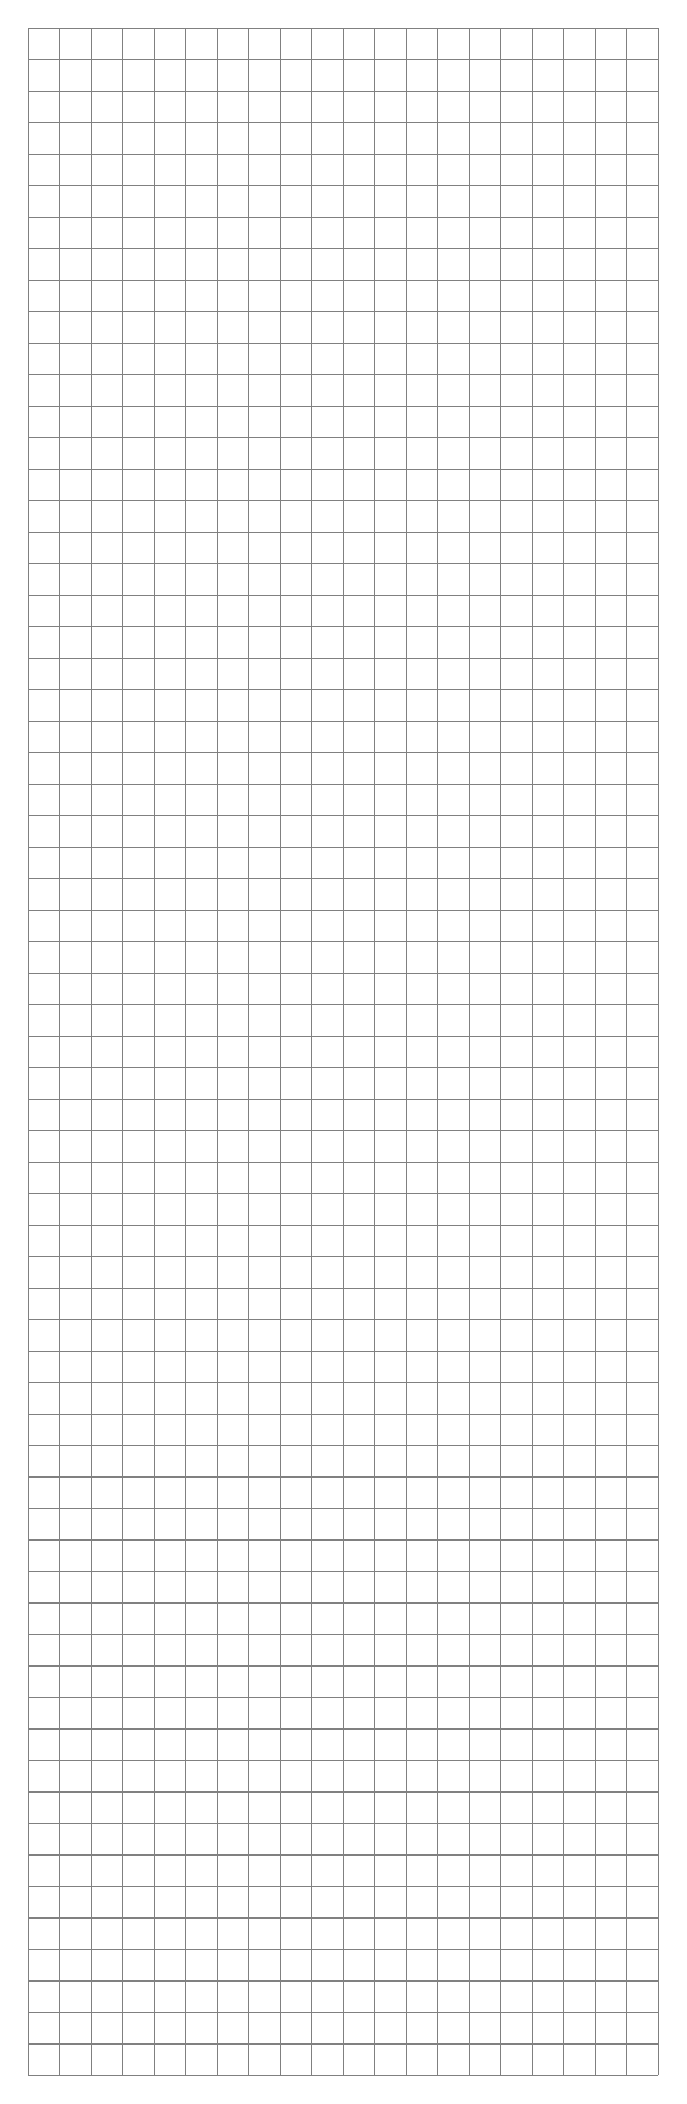
\begin{tikzpicture}[every node/.style={minimum size=1cm-\pgflinewidth, outer sep=10pt}, scale=2]
    \draw[step=0.2cm,color=gray] (0,0) grid (4,13);
    %\draw[step=1cm,color=black,line width=0.4mm] (0,0) grid (4,13);
\end{tikzpicture}


\clearpage
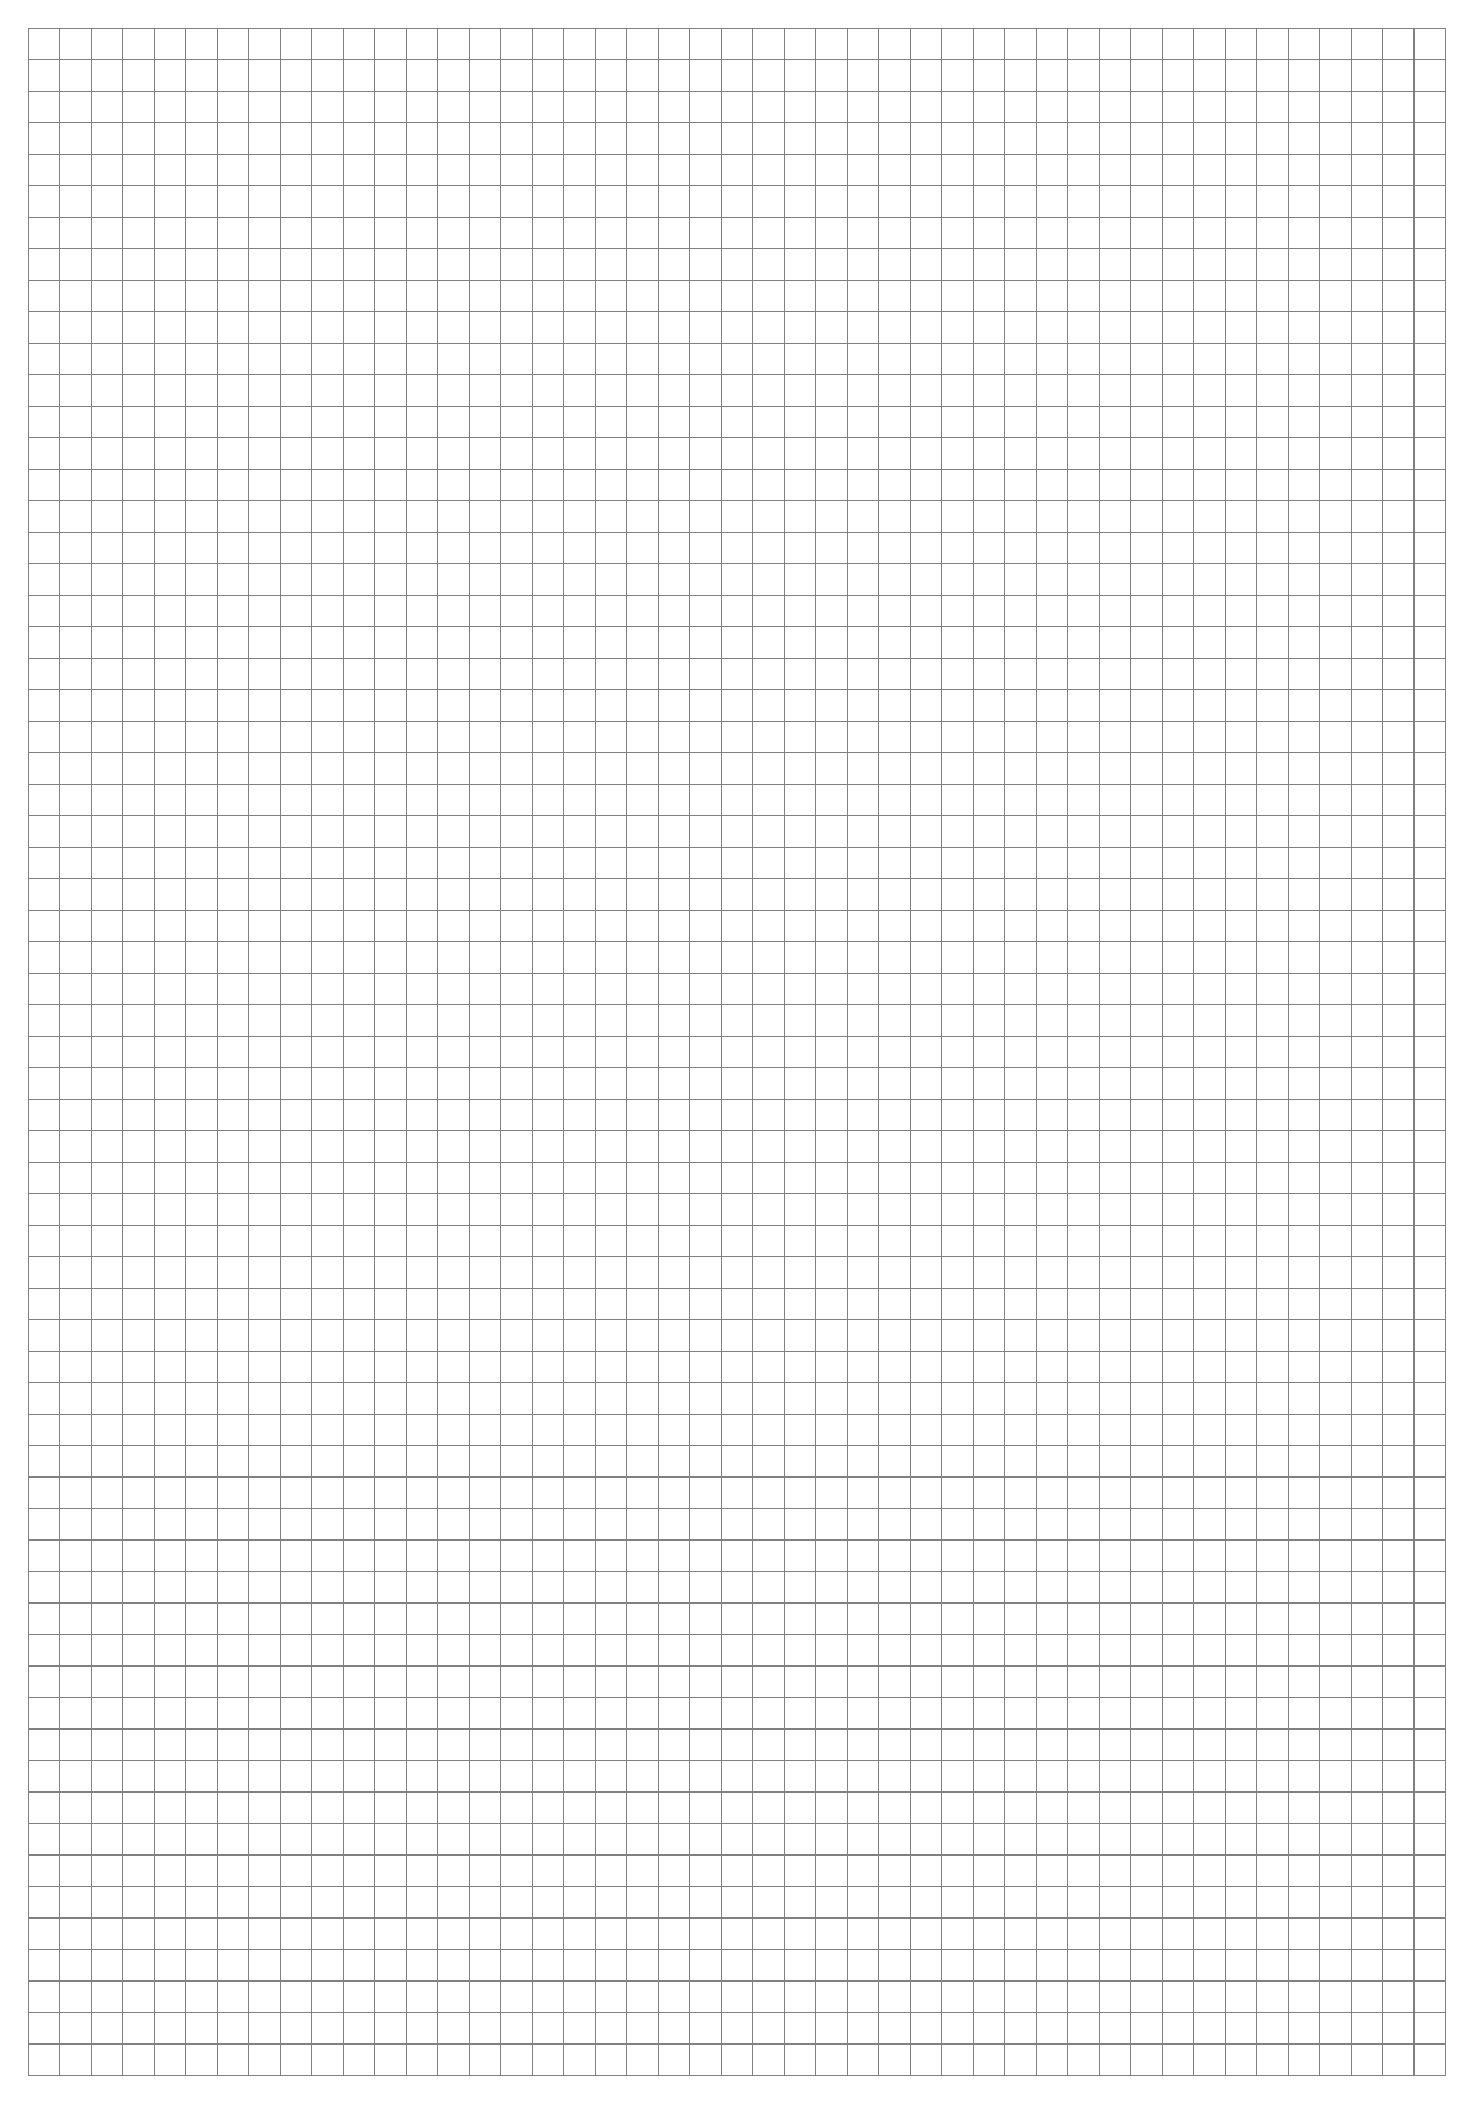
\begin{tikzpicture}[every node/.style={minimum size=1cm-\pgflinewidth, outer sep=10pt}, scale=2]
    \draw[step=0.2cm,color=gray] (0,0) grid (9,13);
    %\draw[step=1cm,color=black,line width=0.4mm] (0,0) grid (4,13);
\end{tikzpicture}

\end{document}

